\section{Dynamic-MSV-Bench and Methodology}
\label{sec:benchmark}

We propose the \textbf{Dynamic-MSV-Bench}, which categorizes multi-shot prompts into two rigorous evaluation scenarios to systematically expose the "Double-Kill" dilemma prevalent in current generative models.

\begin{figure*}[t]
    \centering
    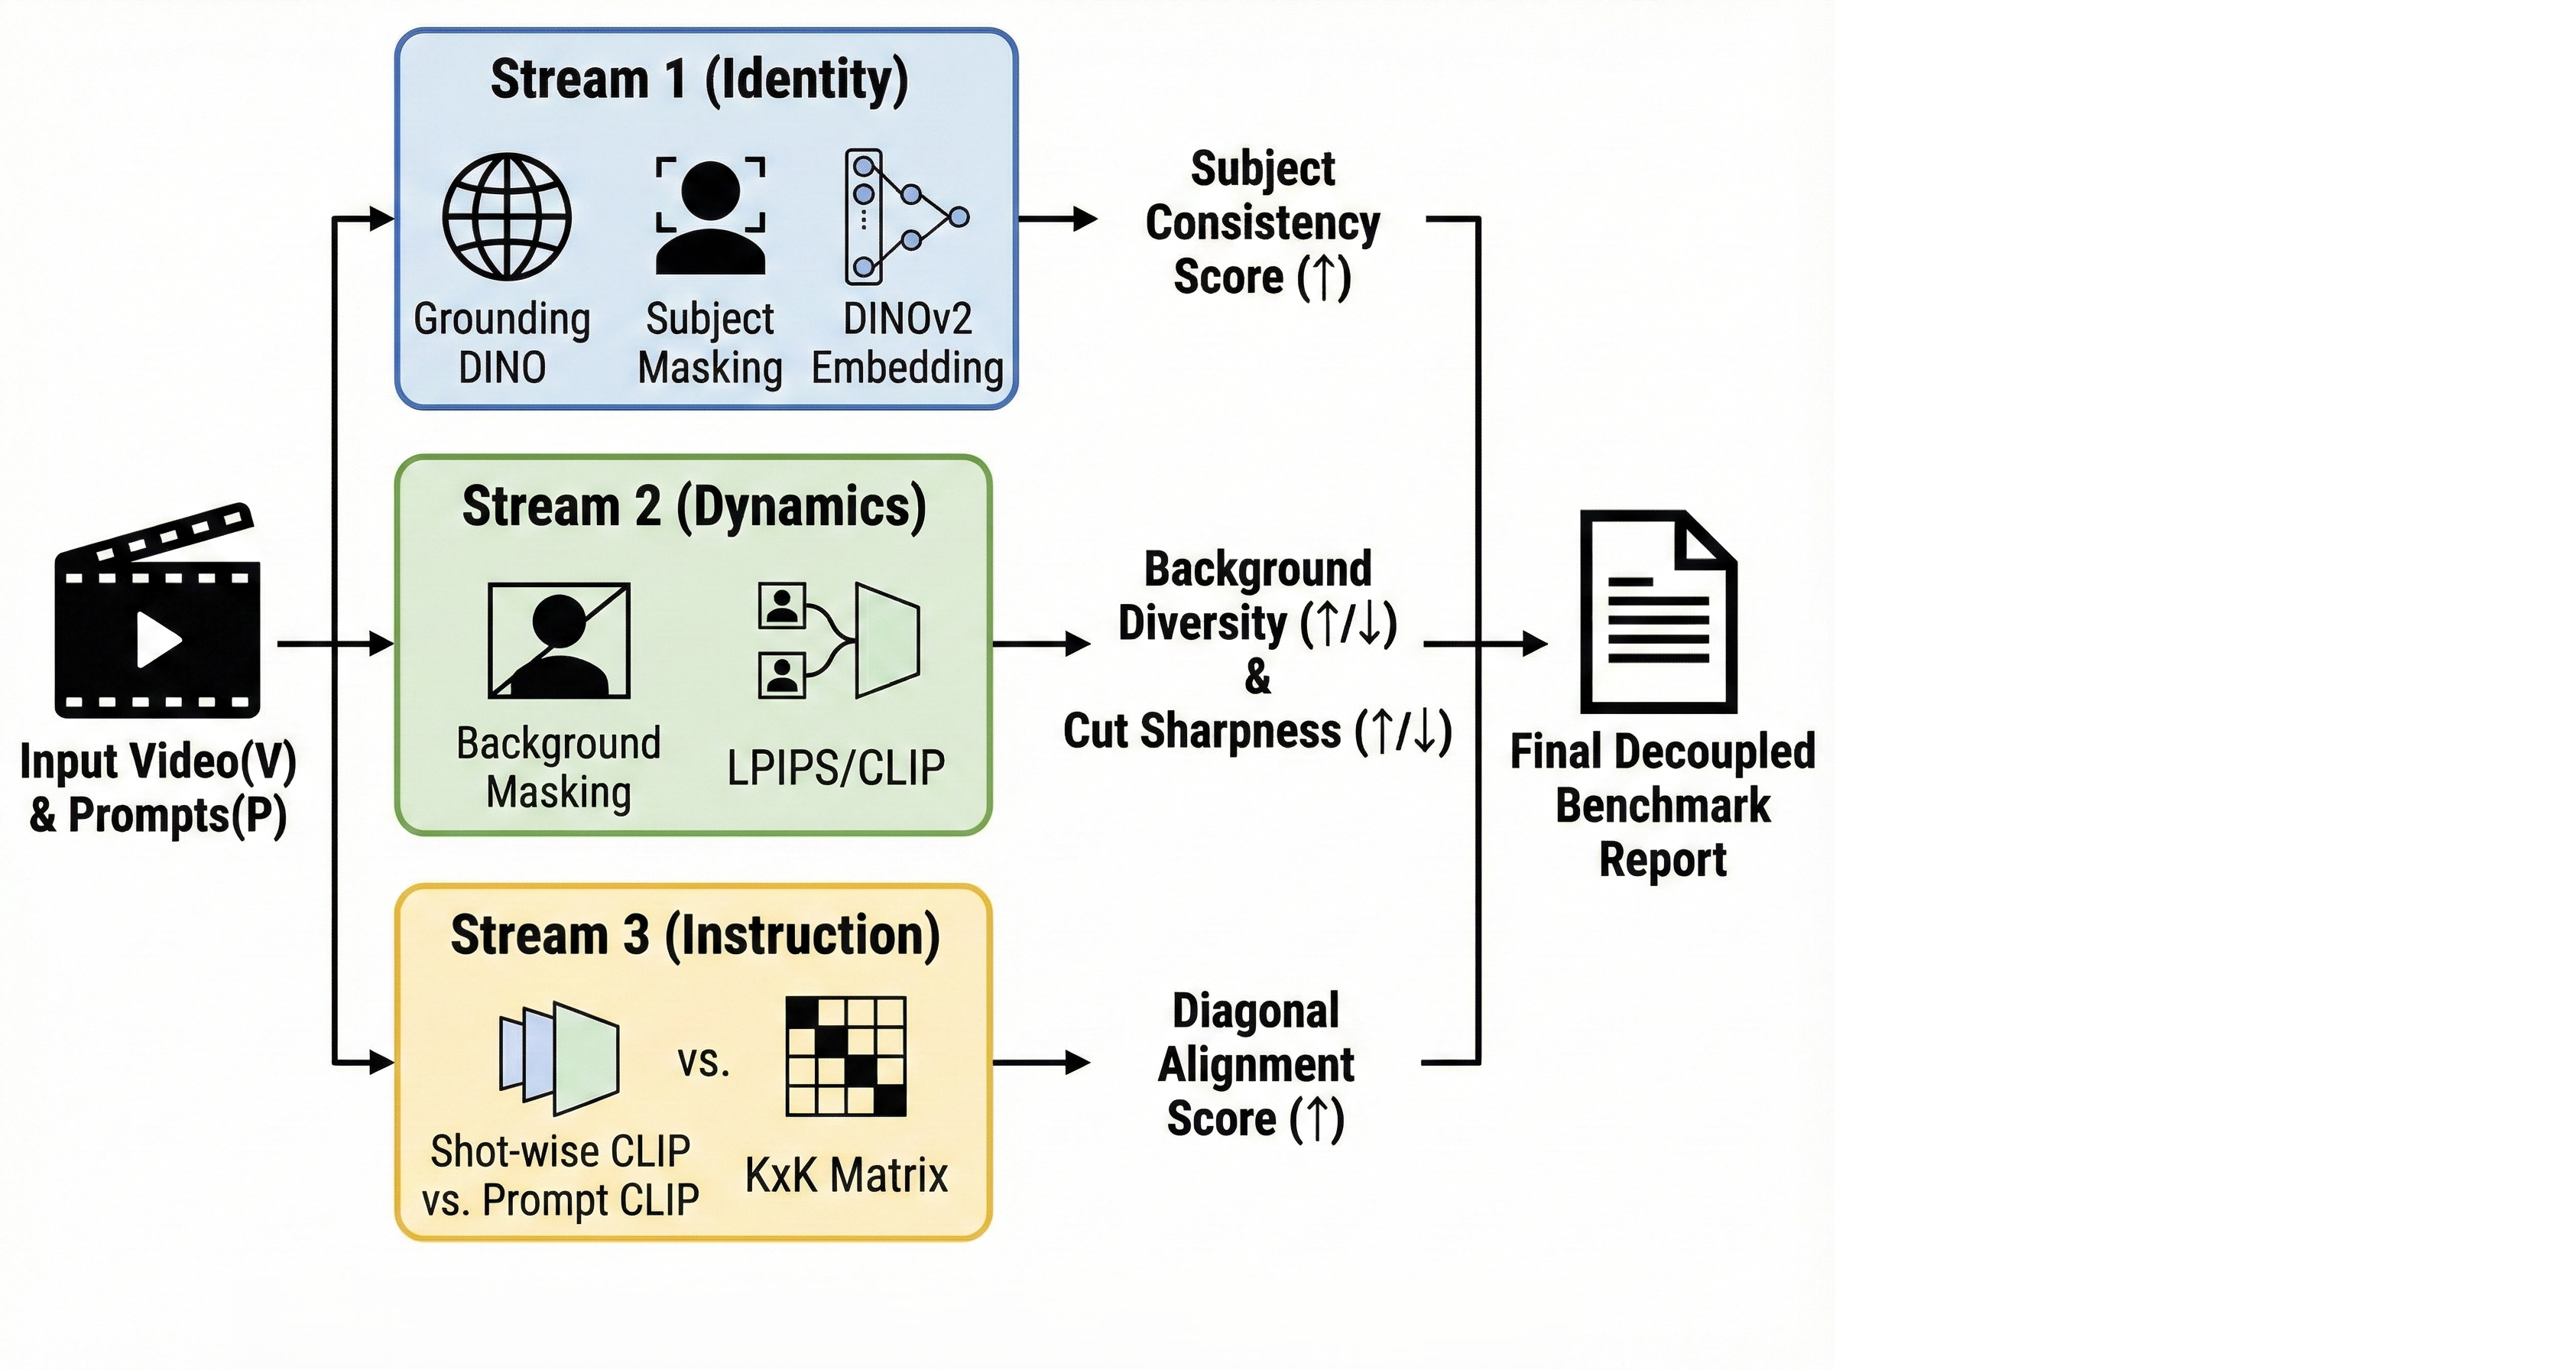
\includegraphics[width=\textwidth]{figures/images/fig2.png}
    \caption{Overview of our Decoupled 4D Evaluation Framework. Unlike holistic metrics like FVD, we process the input video through three independent streams to measure Subject Identity, Background Dynamics/Continuity, and Instruction Following (Diagonal Alignment) separately. This decoupling allows for scenario-aware evaluation (Track S vs. Track M).}
    \label{fig:framework}
\end{figure*}

\subsection{Evaluation Scenarios: Track S and Track M}
As illustrated in Figure~\ref{fig:sets_comparison}, our evaluation framework categorizes generation scenarios into two conceptually orthogonal extremes to stress-test narrative robustness and spatial coherence.

\begin{figure*}[t]
    \centering
    \includegraphics[width=\textwidth]{figures/images/fig_AB.jpg}
    \caption{Conceptual comparison of our two evaluation tracks. (Left) \textbf{Track S: Semantic Leap} tests narrative diversity, requiring radical environment changes while preserving the subject. (Right) \textbf{Track M: Motion Continuity} evaluates spatial integrity, where the background must remain consistent while the camera executes specific motions.}
    \label{fig:sets_comparison}
\end{figure*}

\noindent\textbf{Track S: Semantic Leap (Narrative Diversity).} This track evaluates the model's ability to maintain a consistent subject while drastically shifting the semantic environment. The \textit{Golden Rule for Track S} is defined as demanding high Background Diversity ($\uparrow$), high Cut Sharpness ($\uparrow$), high Subject Consistency ($\uparrow$), and high Diagonal Semantic Alignment (DSA, $\uparrow$). Since the narrative requires a leap between disparate locations, the model must exhibit high variance in its environmental rendering; a low score here directly exposes the \textit{Static Trap}. Furthermore, these environmental jumps should be depicted as distinct cinematic cuts, preventing unnatural "morphing" artifacts. Despite these radical changes, the identity of the main protagonist must remain strictly preserved. Finally, the model must explicitly follow the unique semantic instructions of each shot, guaranteeing the shift is driven by the prompt rather than context bleeding.

\noindent\textbf{Track M: Motion Continuity (Spatial Integrity).} Track M tests physical instructions while keeping the background spatially stable. The \textit{Golden Rule for Track M} demands low Background Diversity ($\downarrow$), low Cut Sharpness ($\downarrow$), high Subject Consistency ($\uparrow$), and high Diagonal Semantic Alignment (DSA, $\uparrow$). The background must remain pixel-consistent while the camera moves; high diversity here indicates \textit{Background Hallucination}. Transitions between camera actions (e.g., from pan to zoom) should be spatially continuous, rewarding a single, cohesive 3D space rather than sharp cuts. Crucially, even with a static background, the model must accurately differentiate between fine-grained camera control instructions, maintaining a high DSA score.

\subsection{Taxonomy of Failure Modes}
Our benchmark uniquely identifies systemic failures by cross-referencing metrics across tracks. Table~\ref{tab:failure_taxonomy} summarizes the key signals used to profile current T2MSV models. The \textbf{Static Trap} is characterized by low diversity but high consistency in both tracks, definitively identified by an artificially low $DSA \approx 0$ due to instruction ignorance. Conversely, \textbf{Identity Amnesia} is identified when models achieve high diversity to satisfy environmental shifts but suffer a catastrophic drop in Subject Consistency.

\begin{table}[ht]
\centering
\caption{Taxonomy of T2MSV Failure Modes. We identify the "Static Trap" and "Identity Amnesia" by analyzing the divergence between Diversity and Consistency across Track S and Track M.}
\label{tab:failure_taxonomy}
\resizebox{\linewidth}{!}{
\begin{tabular}{l|ccc}
\toprule
\textbf{Failure Mode} & \textbf{Track S (Leap)} & \textbf{Track M (Continuity)} & \textbf{Key Metric Signal} \\
\midrule
\textbf{Static Trap} & Div. $\downarrow$, Cons. $\uparrow$ & Div. $\downarrow$, Cons. $\uparrow$ & $DSA \approx 0$ (Both) \\
\textbf{Identity Amnesia} & Div. $\uparrow$, Cons. $\downarrow$ & Div. $\uparrow$, Cons. $\downarrow$ & Cons. $\downarrow$ in Track S \\
\midrule
\textbf{Ideal Target} & Div. $\uparrow$, Cons. $\uparrow$ & Div. $\downarrow$, Cons. $\uparrow$ & High $DSA$ (Both) \\
\bottomrule
\end{tabular}}
\end{table}

\subsection{Formulation of 4D Decoupled Metrics}
Our framework utilizes four specialized indices to quantitatively decompose the generative performance of T2MSV models, explicitly decoupling subject dynamics from environmental rendering.

\noindent\textbf{Subject Consistency ($\mathcal{C}_{subj}$).} We utilize a masked DINOv2~\cite{oquab2023dinov2} similarity to rigorously measure identity preservation across $K$ shots. Let $s_i$ be the representative frame of shot $i$, and $m_i$ be the corresponding subject mask. The score is defined as the mean pairwise cosine similarity between masked embeddings:
$$\mathcal{C}_{subj} = \frac{2}{K(K-1)} \sum_{i < j} \cos(\Phi_{DINO}(s_i \odot m_i), \Phi_{DINO}(s_j \odot m_j))$$

\noindent\textbf{Background Diversity ($\mathcal{D}_{bg}$).} To formally identify the \textit{Static Trap}, we measure the variance of the background environment embeddings ($\overline{m}_i = 1 - m_i$). $\mathcal{D}_{bg}$ is calculated as the mean perceptual distance from the average background embedding:
$$\mathcal{D}_{bg} = 1 - \left( \frac{1}{K^{2}}\sum_{i,j} \cos(\Phi(s_{i}\odot\overline{m}_{i}), \Phi(s_{j}\odot\overline{m}_{j})) \right)$$

\noindent\textbf{Cut-Transition Sharpness ($\mathcal{S}_{cut}$).} We quantify the distinctness of cinematic shot boundaries using Local Perceptual Image Patch Similarity (LPIPS) distance peaks. For a triggered cut at time $t_{cut}$, the sharpness is given by:
$$\mathcal{S}_{cut} = \text{LPIPS}(f_{t_{cut}-1}, f_{t_{cut}+1})$$

\noindent\textbf{Diagonal Semantic Alignment (DSA).} Our core algorithmic novelty measures independent adherence to shot-level instructions, neutralizing the Global Similarity Paradox. We apply a column-wise softmax with logit scaling $\tau$ to the shot-prompt CLIP similarity matrix $M$, generating a probability matrix $P$:
$$P_{i,j} = \frac{\exp(\tau \cdot M_{i,j})}{\sum_{k=1}^{K} \exp(\tau \cdot M_{k,j})}, \quad DSA = \max \left( 0, \frac{\frac{1}{K}\sum_{i=1}^{K} P_{i,i} - \frac{1}{K}}{1 - \frac{1}{K}} \right)$$
As visualized in Figure~\ref{fig:dsa_heatmaps}, a strictly static video yields a DSA of exactly $0.0$, formally penalizing failure to transition.

\begin{figure*}[t]
    \centering
    \includegraphics[width=\textwidth]{figures/dsa_heatmaps_phd.pdf}
    \caption{Diagonal Semantic Alignment (DSA) Heatmaps. (A) Models in the \textbf{Static Trap} exhibit a uniform probability distribution across prompts. (B) Models suffering from \textbf{Context Bleeding} exhibit noisy diagonal alignment. (C) An \textbf{Ideal Decoupled Model} achieves sharp, precise diagonal alignment, proving independent shot execution.}
    \label{fig:dsa_heatmaps}
\end{figure*}